\documentclass[tikz,border=8pt]{standalone}
% Shared look for every TikZ diagram. Load with \input{../../tools/tikz-style.tex}
\usepackage[T1]{fontenc}
\usepackage{lmodern}
\renewcommand{\sfdefault}{lmr}  % diagrams use the same serif as the text
\usetikzlibrary{arrows.meta, positioning, shapes.geometric, calc, fit, backgrounds}
\definecolor{cblue}{HTML}{4C78A8}
\definecolor{corange}{HTML}{F58518}
\definecolor{cgreen}{HTML}{54A24B}
\definecolor{cred}{HTML}{E45756}
\definecolor{cpurple}{HTML}{B279A2}
\definecolor{cgrey}{HTML}{6B6B6B}
\tikzset{
  every picture/.style={font=\sffamily, line width=1.2pt},
  box/.style={draw=#1, fill=#1!12, rounded corners=4pt, align=center, inner sep=7pt, minimum height=1.1cm},
  box/.default=cgrey,
  arrow/.style={-{Stealth[length=3mm]}, draw=cgrey, line width=1.4pt},
  title/.style={font=\sffamily\bfseries\Large},
  note/.style={font=\sffamily\small, text=cgrey, align=center},
}
\AtBeginDocument{\hyphenpenalty=10000 \exhyphenpenalty=10000}

% Order of events: start in x0; control u1 moves the robot to x1; then measurement z1 is read in x1; and so on.
% Controls change the state; measurements only report on it. Hallway run of the chapter in the bottom row.
\begin{document}
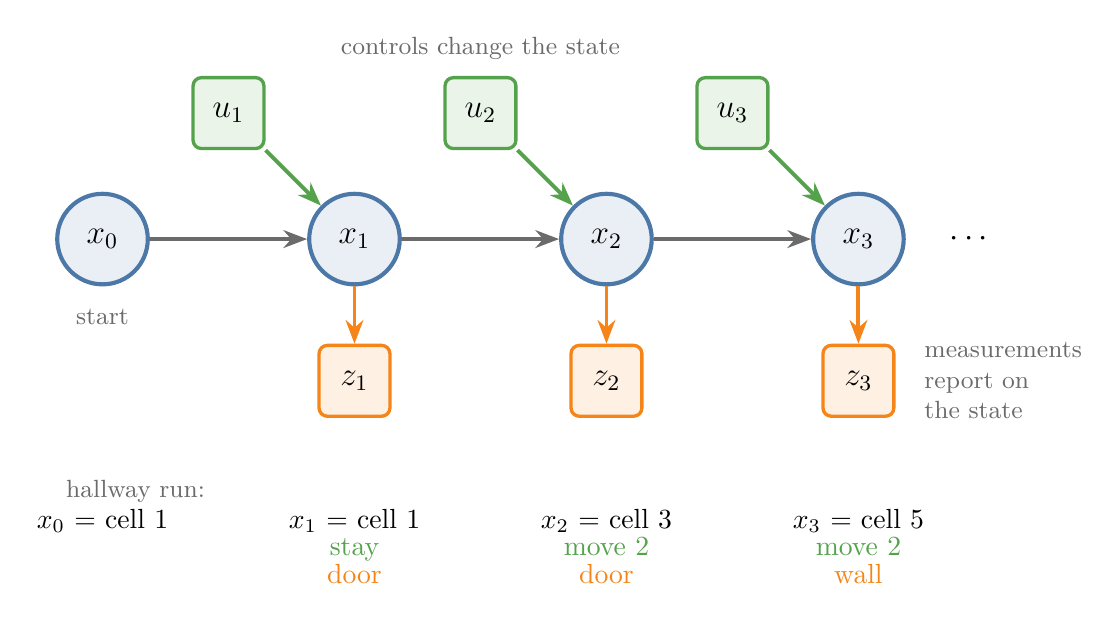
\begin{tikzpicture}[every node/.append style={font=\large}]
  \foreach \t/\x in {0/0,1/3.2,2/6.4,3/9.6} {
    \node[draw=cblue, fill=cblue!12, circle, minimum size=1.15cm, line width=1.5pt] (x\t) at (\x,0) {$x_{\t}$};
  }
  \foreach \t/\x in {1/3.2,2/6.4,3/9.6} {
    \node[draw=cgreen, fill=cgreen!12, rounded corners=3pt, minimum size=0.9cm] (u\t) at (\x-1.6,1.6) {$u_{\t}$};
    \node[draw=corange, fill=corange!12, rounded corners=3pt, minimum size=0.9cm] (z\t) at (\x,-1.8) {$z_{\t}$};
    \draw[arrow, draw=cgreen] (u\t) -- (x\t);
    \draw[arrow, draw=corange] (x\t) -- (z\t);
  }
  \draw[arrow] (x0) -- (x1); \draw[arrow] (x1) -- (x2); \draw[arrow] (x2) -- (x3);
  \node at (11.0,0) {$\cdots$};
  \node[cgreen, note, anchor=south] at (4.8,2.15) {controls change the state};
  \node[corange, note, anchor=west, align=left] at (10.3,-1.8) {measurements\\report on\\the state};
  \node[cblue, note, anchor=north] at (0,-0.75) {start};
  % corridor run
  \node[note, anchor=west, align=left] at (-0.6,-3.2) {hallway run:};
  \foreach \t/\x/\xs/\us/\zs in {0/0/{cell 1}/{}/{}, 1/3.2/{cell 1}/{stay}/{door}, 2/6.4/{cell 3}/{move 2}/{door}, 3/9.6/{cell 5}/{move 2}/{wall}} {
    \node[font=\normalsize, align=center] at (\x,-3.9) {$x_{\t}$ = \xs\\[-2pt]{\color{cgreen}\us}\\[-2pt]{\color{corange}\zs}};
  }
\end{tikzpicture}
\end{document}
